\documentclass[tikz,border=8pt]{standalone}
\usetikzlibrary{arrows.meta,positioning}
\begin{document}
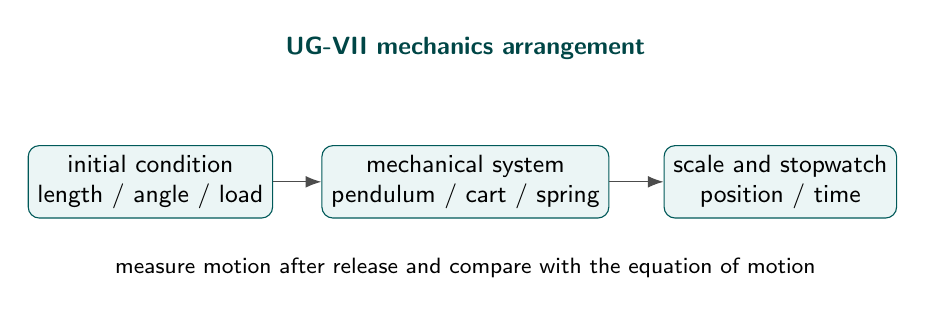
\begin{tikzpicture}[box/.style={draw=teal!70!black,fill=teal!8,rounded corners,minimum width=2.7cm,minimum height=.9cm,align=center,font=\sffamily\small},a/.style={-{Latex[length=2mm]},draw=black!70}]
\node[font=\sffamily\bfseries\small,text=teal!55!black] at (0,1.7) {UG-VII mechanics arrangement};
\node[box] (i) at (-4,0) {initial condition\\length / angle / load};
\node[box] (s) at (0,0) {mechanical system\\pendulum / cart / spring};
\node[box] (m) at (4,0) {scale and stopwatch\\position / time};
\draw[a] (i)--(s); \draw[a] (s)--(m);
\node[font=\sffamily\footnotesize] at (0,-1.1) {measure motion after release and compare with the equation of motion};
\end{tikzpicture}
\end{document}

